\section{Futures} \label{sec:futures}
Consider a mock-up parallel arrow combinator:
\begin{code}
someCombinator :: (Arrow arr) => [arr a b] -> [arr b c] -> arr [a] [c]
someCombinator fs1 fs2 = parEvalN () fs1 >>> rightRotate >>> parEvalN () fs2
\end{code}

In a distributed environment, a resulting arrow of this combinator first evaluates all |[arr a b]| in parallel, sends the results back to the master node, rotates the input once and then evaluates the |[arr b c]| in parallel to then gather the input once again on the master node.
Such situations arise, \eg in scientific computations when the data distributed across the nodes needs to be transposed. A concrete example is 2D FFT computation \cite{Gorlatch,Berthold2009-fft}.

While the above example could be rewritten into only one |parEvalN| call by directly wiring the arrows together before spawning, it illustrates an important problem. When using a |ArrowParallel| backend that resides on multiple computers, all communication between the nodes is done via the master node, as shown in the Eden trace in Figure~\ref{fig:withoutFutures}. This can become a serious bottleneck %in heavy threaded applications.
for larger amount of data and number of processes \citep[as \eg][showcases]{Berthold2009-fft}.
\begin{figure}[ht]
	\centering
	\includegraphics[width=0.9\textwidth]{images/withoutFutures}
	\caption[without Futures]{Communication between 4 Eden processes without Futures. All communication goes through the master node. Each bar represents one process. Black lines between processes represent communication. Colors: blue $\hat{=}$ idle, green $\hat{=}$ running, red  $\hat{=}$ blocked, yellow $\hat{=}$ suspended.}
	\label{fig:withoutFutures}
\olcomment{more practical and heavy-weight example! fft (I have the code)?}\\
\mbcomment{Depends... Are the communications easy to read in such an example?}\\
\mbcomment{Keep the description for the different colours, or link to
  the EdenTV description in \ref{sec:edentv}}
\olcomment{ok as is}
\olcomment{use the fft example (when it works)?}
\end{figure}

This is in fact only a problem in distributed memory (in the scope of this paper) and we should  allow nodes to communicate directly with each other. Eden already ships with "remote data" that enable this \cite{AlGo03a,Dieterle2010}.
But as we want code with our DSL to be implementation agnostic, we have to wrap this context. We do this with the |Future| typeclass (Fig.~\ref{fig:future}).
\begin{figure}[h]
\begin{code}
class Future fut a | a -> fut where
    put :: (Arrow arr) => arr a (fut a)
    get :: (Arrow arr) => arr (fut a) a
\end{code}
\caption{Definition of the |Future| typeclass.}
\label{fig:future}
\end{figure}
Since |RD| is only a type synonym for a communication type that Eden uses internally, we have to use some wrapper classes to fit that definition, though, as Fig.~\ref{fig:RDFuture} shows. %This is due to the same reason we had to introduce a wrapper for |Strategy a| in the GpH Haskell implementation of |ArrowParallel| in Section~\ref{sec:parrows:multicore}.
Technical details are in Appendix, in Section~\ref{app:omitted}.

For the |Par| Monad and GpH Haskell backends, we can simply use |BasicFuture|s (Fig.~\ref{fig:BasicFuture}), which are just simple wrappers around the actual data with boiler-plate logic so that the typeclass is satisfied. This is because the concept of a |Future| does not change anything for shared-memory execution as there are no communication problems to fix, but we require a common interface so the parallel Arrows are portable across backends.
\begin{figure}[tb]
\begin{code}
data BasicFuture a = BF a

instance (NFData a) => NFData (BasicFuture a) where
    rnf (BF a) = rnf a

instance (NFData a) => Future BasicFuture a where
    put = arr BF
    get = arr (\(BF a) -> a)
\end{code}
\caption{The |BasicFuture| type and its |Future| instance for the |Par| Monad and GpH Haskell backends.}
\label{fig:BasicFuture}
\end{figure} % $


In our communication example we can use this |Future| concept for direct communication between nodes as shown in Fig.~\ref{fig:someCombinatorParallel}.
\begin{figure}[tbh]
\begin{code}
someCombinator :: (Arrow arr) => [arr a b] -> [arr b c] -> arr [a] [c]
someCombinator fs1 fs2 =
	parEvalN () (map (>>> put) fs1) >>>
	rightRotate >>>
	parEvalN () (map (get >>>) fs2)
\end{code}
\caption{The mock-up combinator in parallel.}
\label{fig:someCombinatorParallel}
\end{figure}
In a distributed environment, this gives us a communication scheme with messages going through the master node only if it is needed---similar to what is shown in the trace visualization in Fig.~\ref{fig:withFutures}. \olcomment{Fig. is not really clear. Do Figs with a lot of load? --- fft?}
\begin{figure}[ht]
	\centering
	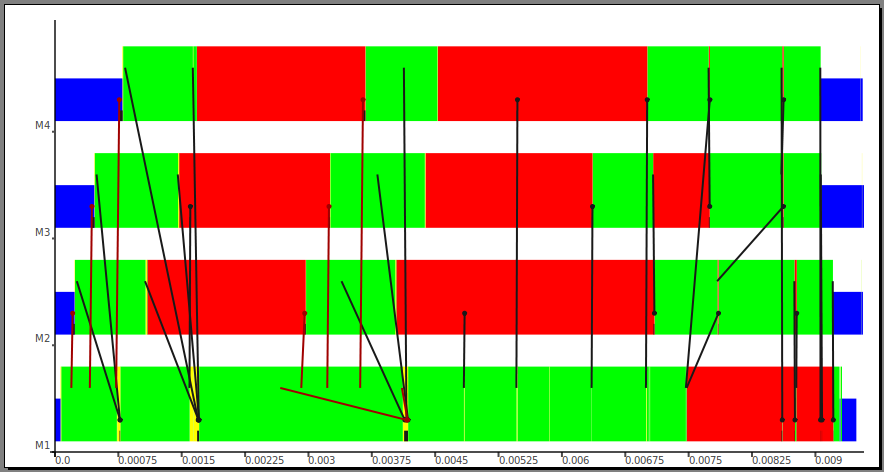
\includegraphics[width=0.9\textwidth]{images/withFutures}
	\caption[with Futures]{Communication between 4 Eden processes with Futures. Other than in Fig.~\ref{fig:withoutFutures}, processes communicate directly (black lines between the bars) instead of always going through the master node (bottom bar).}
	\label{fig:withFutures}
\end{figure}
